%\subsubsection*{Las herramientas que adquieren datos}
El grado de avance que ha experimentado la tecnología en general, y la electrónica en particular, gracias a la industria de los semiconductores, permite que la producción científica pueda adquirir una gran cantidad de datos. Esto, requiere el relevamiento y registro de diferentes tipos de magnitudes físicas y/o químicas sobre el objeto o proceso sobre el que se está investigando. Sin embargo, esta no es una tarea simple ya que, en muchos casos, estas magnitudes son difíciles de observar y cuantificar con los sentidos de un operador. Entonces, se vuelve conveniente transformar las variables a medir en otras que resulten más simples.\\

El dispositivo que recibe estímulos energéticos de una condición, situación o fenómeno físico y/o químico y los convierte en una señal asociada y definida de otra forma de energía, se lo denomina transductor\cite{Pallas-Areny2001}\cite{considine1971encyclopedia}. En otras palabras, este tipo de máquinas son conversores de energías\cite{considine1971encyclopedia}\cite{Pallas-Areny2001}\cite{PerezGarcia2008}. Un sensor es un tipo especial de transductores que posee como variable de salida una señal eléctrica que está adaptada para ser ingresada en un circuito electrónico, o adecuada al sistema de medida que se utilice \cite{Fraden2010}\cite{Slawinski2011}\cite{Ogata2002}.\\

Las altas escalas de integración de circuitos alcanzadas (aún en incremento) posibilitan el diseño de sistemas sensoriales cada vez más complejos, en los cuales se logra agrupar miles de sensores en áreas reducidas, obteniendo medidas simultáneas y flujos crecientes de datos. Uno de los desarrollos que se encuentra en boga es el de sensores y sistemas que adquieran imágenes de diferentes tipos. Desde el punto de vista digital, una imagen es un arreglo bidimensional de números, los cuales pueden ser exhibidos en una pantalla en forma de intensidad y colores de luz. Por esto, un sensor de imagen puede estar compuesto, bien por un arreglo bidimensional de sensores lumínicos, por un transductor que es simultáneamente desplazado y medido, o por una combinación de ambos métodos. En todo caso, es de suma utilidad que la lectura de imágenes sea realizada en el menor tiempo posible ya que cada imagen conlleva una cantidad no menor de datos.\\

%TODO insertar aquí ejemplos de desarrollo de sensores de imágenes
Uno de los trabajos más importantes en este sentido, fue el desarrollo de los CMOS APS ({\it Active Pixel Array}, o matriz de pixeles activos) \cite{Mendis1994}. La Figura \ref{fig:pix} muestra un dibujo esquemático del funcionamiento de cada uno de los pixeles activos que componen la matriz. Este posee un fotodiodo, que es el elemento transductor. En un primer momento, este diodo es conectado en forma inversa, generando una región de vaciamiento entre sus terminales. Luego, cuando un fotón incide sobre él, se forman pares electrón-hueco y ellos circulan a través del diodo a las terminales, generando una pequeña caída de tensión. Finalmente, se mide la tensión del diodo, cuya intensidad será inversamente proporcional a la cantidad de fotones que incidieron sobre el pixel en cuestión.

\begin{figure}[ht]
	\caption{Esquema de un pixel activo}
	\label{fig:pix}
\end{figure}

A partir del desarrollo de los APS, se fue perfeccionando el método hasta obtener integrados con mayor cantidad de pixeles y para lograr aplicaciones específicas basadas en este fenómeno. Por ejemplo, en los trabajos \cite{Hu-Guo2009} y \cite{Baudot2009} se presentan sensores CMOS basados en la arquitectura MIMOSA (de {\it Minimum Ionizing particule MOS Active pixel Sensor}, Sensor con Pixel activo MOS de particulas ionizantes mínimas). Estos sensores se desarrollaron con el objetivo específico de detección de radiación. En otro trabajo, Hizawa y otros \cite{Hizawa2007} fabricaron un sensor que adquiere imágenes midiendo el pH de en cada uno de los pixeles, obteniendo imágenes de fenómenos químicos en tiempo real.\\

Desde un punto de vista electrónico, para poder transmitir grandes volúmenes de datos en forma digital, se requiere de circuitos que sean capaces de operar a altas frecuencias de conmutación. Esto no es trivial, ya que cuando las longitudes de onda que se mueven a través de un circuito son comparables con sus dimensiones físicas, se evidencian capacidades e inductancias parásitas no contempladas que perjudican el desempeño de los sistemas. Por ejemplo, si se desea transmitir datos en serie con una variación entre sus datos de \SI{300} {\mega\hertz}, se habla de ondas cuya longitud de onda es de \SI{1}{\meter}. Se dice que las dimensiones son comparables cuando el largo del conductor posee al menos un cuarto de la longitud de onda, es decir, para este caso, \SI{25}{\centi\meter}. Si bien esto puede parecer grande, se debe notar que a mayores frecuencias, este efecto comienza a ser aún más perjudicial.\\

Otro problema que presentan los circuitos de alta velocidad tiene que ver con los tiempos de propagación de las corrientes y tensiones que circulan a través de ellos. Cuando se aplica un impulso en un conductor, la onda viaja a la velocidad de la luz. Esto quiere decir que la tensión no llega al mismo tiempo a todos los puntos del circuito, sino que, mientras más alejada está la fuente, más lejos está se demora en responder. Puede suceder, entonces, que la lógica del circuito se demore más que el pulso de reloj que indica un cambio de estado, obteniendo así un comportamiento no deseado, si no está correctamente diseñado y contemplado este aspecto.\\

Una solución para los circuitos electrónicos que necesitan mover grandes volúmenes de datos, puede ser la incorporación varios conductores a través de los cuales puede fluir la información. Retornando al ejemplo de los datos transmitidos con variaciones de hasta \SI{300}{\mega\hertz}, si son enviados a través de dos conductores, la frecuencia necesaria cae a \SI{150}{\mega\hertz}, con 3, se obtiene una reducción de la frecuencia a \SI{100}{\mega\hertz}, con 10, es suficiente con \SI{30}{\mega\hertz}, etc. La cantidad de conductores a través de los cuales circula la información, se denomina ancho de bus.\\

En gran medida, la incorporación y evolución de microcontroladores permite obtener una captura y obtención cada vez superior de datos. Sin embargo, este tipo de dispositivos poseen una estructura rígida, capacidad de procesamiento limitada a una instrucción por vez y ancho de bus definido, la única opción para aumentar los volúmenes de datos que circulan a través de ellos, es un aumento de la frecuencia de funcionamiento, generando los problemas anteriormente detallados. Una solución óptima, sin considerar los costos asociados a esto, sería el desarrollo de un circuito integrado de aplicación específica (ASIC del inglés{\it Application Specific Integrated Circuit}). En este tipo de circuitos, el diseñador elabora un circuito que puede correr a altas velocidades y, a su vez, obtener un ancho de bus sin restricciones, más que las dimensiones físicas del área donde será realizado el circuito. Sin embargo, cuando sí se considera el costo asociado a este enfoque, se vuelve una solución ineficiente en bajas cantidades. La manufactura de este tipo de dispositivos cuesta desde €2500, en los procesos más económicos, hasta cientos de miles de dólares. Gran parte de estos costos son no recurrentes, es decir, solo se pagan una vez por proyecto. En grandes volumenes, este tipo de soluciones se vuelven más convenientes.\\

Otro enfoque, es la utilización de Arreglos de Compuertas Programables por Campo (FPGA, acrónimo del inglés {\it Field-Programmable Gate Array})para realizar el desarrollo. Un FPGA es un dispositivo electrónico que posee la capacidad de sintetizar casi cualquier circuito digital. En esencia, es una matriz de bloques lógicos (también llamadas {\it slices} o celdas lógicas, dependiendo del fabricante), que contienen Tablas de Verdad(LUTs o {\it Look-Up-Table}) y flip-flops (ff), entre otras cosas, y pueden ser interconectadas entre sí, según el criterio del usuario. Así, permite implementar una solución digital en un circuito físico, a diferencia del microcontrolador que lo realiza a través de un algoritmo. Esto, incorpora la ventaja de definir el ancho de bus necesario para relevar una gran cantidad de datos y transmitirlos a frecuencias de trabajo menores, además de ejecutar tareas en paralelo, disminuyendo los tiempos de procesamiento. A su vez, al ser implementado en un área muy pequeña, debido a la integración del sistema, puede trabajar a frecuencias muy elevadas, lo que implica una mayor tasa de datos aún. Los costos de un FPGA, dependiendo de las prestaciones, van desde U\$S 1 a U\$S \SI{50000}{}. A pesar de la gran diversidad de precios existentes en el mercado, una FPGA de bajo costo suele tener muy buenas prestaciones para la mayor parte de las aplicaciones.\\

Existen diversas publicaciones en donde se observa el uso de FPGAs para la implementación de sistemas que producen imágenes. Por ejemplo, el desarrollo de un sensor de radiación utilizando una cámara CMOS comercial. Para ello, los autores utilizaron un FPGA para configurar y transmitir imagenes a un grabador de video a través de puerto UART. Esto permitió adquirir una imagen accionando un disparador realizado con un pulsador\cite{Perez2017}.\\

Se denomina ultrasonografía a la técnica de adquirir imágenes basandose en reflexiones de ultrasonido. Sus aplicaciones son múltiple, en las que se destaca el diagnóstico médico, ya que es una técnica no invasiva y sin riesgos de radiación ionizante sobre el paciente. Un trabajo reciente desarrolló un sistema de ecografía médica con bajo costo utilizando un FPGA\cite{biswas2018embedded}. El autor también presentó un algoritmo realizado y probado en PC. Luego se implementó e en una FPGA.\\

Yanagisawa, entre otros, desarrolló un sistema con telescopios pequeños para explorar objetos de campo cercano con la finalidad de monitorear cuerpos celestes que puedan colisionar con el planeta\cite{Yanagisawa2018}. Los autores utilizan la velocidad de los circuitos implementados en FPGA para minimizar el tiempo de adquisición.\\

La obtención de datos por si misma no otorga información. Para ello, es probable que un gran flujo de datos requiera de un procesamiento y análisis exhaustivo de los mismos. La invención y evolución de las computadoras, como así también el desarrollo de nuevos algoritmos, dan lugar a procesamiento de datos cada vez más complejos en tiempos mucho menores.\\

Las primeras ENIAC, computadora de propósito general desarrollada en el año 1946 para el cálculo de tablas balísticas de las fuerzas armadas estadounidenses, podía ejecutar 20 operaciones cada \SI{10}{\micro\second} \cite{Goldstine1946}, es decir, ejecutaba instrucciones con una frecuencia máxima de \SI{200}{\kilo\hertz}. A su vez, tuvo un costo aproximado de U\$S 500.000, pesaba 5 t y consumía \SI{175}{\kilo\watt}.\\

En contraste con aquello, es posible conseguir en el mercado actual, computadoras cuyas dimensiones y peso hacen que puedan ser levantadas con las manos, ejecutan instrucciones en cuenstión de nanosegundos, (5 ordenes de magnitud menos), consumen menos de \SI{1}{\kilo\watt} y cuestan algunos cientos de U\$S. A tal punto ha evolucionado esta tecnología que se encuentran presente computadoras muy potentes en casi cualquier laboratorio, oficina u hogar. Esta potencia de cálculo, ayudado por el desarrollo de nuevos métodos y algoritmos de cálculo, permiten a los investigadores procesar miles de datos en tiempos muy reducidos, ayudando al análisis de los mismos y la obtención de información.\\

La generación de datos y el procesamiento de lo mismos se da en sistemas diferentes. Ellos requieren, por tanto, de una conexión a través de la cual los datos puedan ser transferidos de un sistema al otro. Se torna de suma utilidad, entonces, proveer una comunicación efectiva y robusta que permita transmitir grandes volúmenes de datos en poco tiempo, y de esta forma facilitar los tiempos de desarrollo, las pruebas y depuración.\\

Implementar un sistema de comunicación en una FPGA, si bien no es trivial, puede ser resuelto de muchas maneras, quedando a criterio del desarrollador utilizar algún protocolo de comunicación estándar, o bien, diseñar uno propio. Sin embargo, desde el punto de vista de una computadora, las comunicaciones se vuelven un poco más estrictas y acotadas a los puertos y señales que puede manejar el equipo, conforme el fabricante haya establecido.\\

Es por eso que este trabajo busca implementar una comunicación entre una computadora personal y una FPGA, utilizando un protocolo estándar, que esté disponible en cualquier computadora comercial y que posea una tasa de bit suficiente para poder transmitir imagenes.\\

%PRESTAR ATENCION: pegado de archivo externo!!!

%ARCHIVO transmitir.tex modificado

%Dada la motivación, se puede decir a priori que el objetivo del presente trabajo es la implementación de una efectiva comunicación entre una Computadora Personal (PC) y una FPGA. Sin embargo, este objetivo tan amplio se plasmará de forma más concreta y detallada en la Sección \ref{int:obj}.\\

Pero, ¿Cuántos datos son suficientes para este propósito? Se toma como base de diseño el sensor que utiliza Pérez en su Tesis de Maestría \cite{Perez2018}, una cámara para adquirir imágenes monocromáticas de código MT9M001C12STM, comercializado por Actina Imaging \cite{MicronTechnology2004} que transmite datos a una tasa de \SI{48}{\mega\bit\per\second}.\\

Además la implementación debe ser compatible con equipos convencionales que se consigan fácilmente en el mercado y no posean especificaciones fuera de las de uso doméstico. Esto se cumple hoy en día con tres tipos de puertos: Ethernet, dedicado principalmente a conexión de redes mediante cables; Wi-Fi, utilizado para el accesos a la red de forma inalámbrica; y USB, especializado en periféricos.\\

Al hablar de Ethernet o Wi-Fi, se hace referencia a dos formas diferentes de conectarse a una misma cosa: una red de computadoras. En otras palabras, se habla de dos o más nodos, compuestos por PC's o cualquier aparato electrónico con capacidad de realizar cálculo binario, que pueden intercambiar datos a través de una trama bastante compleja de componentes diferentes. Ambos protocolos hacen referencia solo a la conexión física de los dispositivos y el control de acceso de cada uno de ellos a la conexión. Quedando a cargo de otro tipo de sistemas, con sus protocolos, que los datos enviados puedan ser correctamente recibidos por el usuario de la PC. La gran diferencia entre ellos radica en el medio físico que utilizan: Wi-Fi emplea ondas electromagnéticas emitidas mediante radiofrecuencia, mientras que en Ethernet, estas ondas son acarreadas por uno o más conductores, como ser cable coaxial, cables de par trenzado o fibra óptica.\\

\begin{figure}
	\centering
	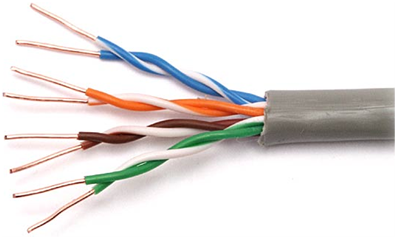
\includegraphics[width=0.4\textwidth]{partrenzado.png}
	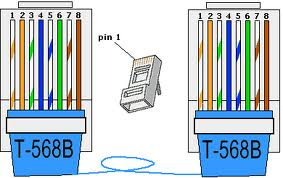
\includegraphics[width=0.4\textwidth]{utp.jpeg}
	\caption{Par Trenzado y un dibujo de su ficha de conexión.}
	\label{fig:utp}
\end{figure}

En particular, el estandar Ethernet, también conocido como IEEE 802.3, es un protocolo que define cómo se deben conectar nodos a través de conductores para conformar red de área local (LAN o {\it Local Area Network}), de forma que puedan transmitir información a velocidades seleccionables entre \SI{1}{\mega\bit\slash\second} y \SI{400}{\giga\bit\slash\second} \cite{Ethernet2018}. Utiliza una tecnología denominada Acceso Múltiple Sensando la Portadora con Detección de Colisiones (CSMA/CD del inglés {\it Carrier Sense Multiple Access with Collision Detection}), la cual antes de transmitir, corrobora que no exista una señal portadora y espera para retransmitir si ésta está presente. Dependiendo de la frecuencia de trabajo y la tasa de transferencia a la que transporta el mensaje, la norma especifica el conector y la distancia máxima a la que debe conectarse una repetidora, es decir, un aparato que reconstruya y emita la señal. Estos conectores pueden ser cable coaxial, fibra optica o cable de par trenzado. Este último es el más usual en las PCs comerciales y se muestra, junto a su ficha característica en la Figura \ref{fig:utp}.\\


Si bien se puede implementar la comunicación vía Ethernet, cumpliendo con las especificaciones propuestas, es muy probable que el único puerto que posea la PC se encuentre conectado a la red y se necesitará una infraestructura mayor para lograr una efectiva comunicación. Por tanto, USB se observa como una solución óptima.\\

A su vez, USB presenta, al día de la fecha, con tres versiones de su norma, con diferentes velocidades: 

\begin{itemize}
	\item La version 1 posee dos revisiones, 1.0 fue lanzada al mercado en el año 1996 y 1.1 que se presentó en Agosto de 1998. Ambas revisiones alcanzan una tasa máxima de \SI{12}{\mega\bit\per\second}. 
	\item USB 2.0 fue presentado en Septiembre del 2000 y es capaz de transmitir \SI{480}{\mega\bit\per\second}.
	\item Dependiendo de la revisión, desde USB 3.0, lanzada al mercado en 2011, que transmite \SI{5}{\giga\bit\per\second}, hasta \SI{20}{\giga\bit\per\second} de la revisión USB 3.2, que fue presentada en 2017.
\end{itemize}

Con estas velocidades, es suficiente para el propósito del siguiente trabajo, la implementación una comunicación USB 2.0, con \SI{480}{\mega\bit\per\second}.\\

\begin{figure}[t]
	\centering
	\begin{tikzpicture}[scale=\textwidth/\paperwidth,>=latex]
	\begin{scope}
	\begin{scope}[transform shape,node distance=2]
	\node[bloque]	(cy)					{Interfaz};
	\node[bloque]	(fpga)	[right=of cy]	{FPGA};
	\node[bloque]	(pc) 	[left=of cy]	{PC};
	\draw[->,thick]	(pc.15)	-- node (usbd+) [above]	{D+} (pc.15 -| cy.west);
	\draw[->,thick]	(cy.195)-- node (usbd-) [below]	{D-} (cy.195 -| pc.east);
	\draw[<->,thick](cy.15) -- node (data) [above] {Datos} (cy.15 -| fpga.west);
	\draw[->,thick]	(fpga.195)	-- node (ctrl) [below]	{Control} (fpga.195 -| cy.east);
	\node[node distance=.4]	(usb text) [above=of usbd+]	{USB};
	\end{scope}
	\begin{scope}
	\node[rectangle,rounded corners,draw=black,dashed,fit=(usb text)(usbd+)(usbd-)(cy.south west)(pc.east)](usb){};
	\end{scope}
	\end{scope}
	\end{tikzpicture}
	\caption{Esquema propuesto para implementar la comunicación}
	\label{fig:esq}
\end{figure}

El alumno sabe que es posible implementar una comunicación USB completa a través de una FPGA. Sin embargo, esto sería muy costoso en términos de tiempos de desarrollo y de recursos de FPGA disponibles para la implementación de otros sistemas, los cuales son el objetivo de la comunicación.\\

Se plantea, entonces, un esquema como el que se observa en la Figura \ref{fig:esq} en la cual se utiliza una interfaz externa al FPGA. La comunicación USB propiamente dicha será efectuada entre la interfaz y la PC, mientras que se plantea una comunicación diferente entre la interfaz y el FPGA. Este último, por su parte, tendrá la tarea de realizar el control de esta comunicación.\\

%Atención con estos parrafos!!!!

%
% una tasa de bit que permita transmitir imagenes y que los puertos sean fácilmente accesibles en PCs comerciales, resaltan tres protocolos que permitirían lograr este cometido: Ethernet, USB y Wi-Fi. Estos protocolos, son los que actualmente se encuentran presente en cualquier aparato nuevo. Estas normas, entre otras, han dejado de lado a estandares que antes eran muy comunes y que algunos periféricos aún cuentan, como ser RS-232 o PS/2, entre otras.\\ 
%
%En una primera aproximación, la que mayor tasa de datos puede proveer, sin dudas es el estandar Ethernet. Estas comunicaciones pueden alcanzar hasta \SI{400}{\giga bp\second}. Sin embargo, la norma Ethernet está principalmente pensada para redes de computadoras, por lo general se dipone de un solo puerto, el cual puede estar conectado a una red de internet y un periférico que tenga este puerto como conexión requerirá de alguna infrastructura adicional con cables más o menos extensos para lograr la comunicación.\\
%
%En el caso de tratar de utilizar una comunicación via Wi-Fi, es posible que se necesite algún enrutador adicional a la hora de conectarse. A su vez, la tecnología inalámbrica con mayor ancho de banda está disponible hace unos pocos años y no todos los equipos cuentan con esta posibilidad, ofreciendo en esos casos una tasa máxima de \SI{54}{\mega bp \second}. La tasa de transmisión real máxima, descontando todos los encabezados y las colas que posee la norma, es de \SI{19}{\mega bp\second}.

%ARCHIVO

%Es por esto que la PC {\it Personal Computer} se ha transformado en la herramienta indispensable en cualquier ámbito, pero en especial en los entornos en donde se requiere el  manejo, cálculo, procesamiento y análisis de grandes cantidades de datos e información.\\
%
%
%
%Desde la inclusión de la norma USB, en el año 1996 a la fecha, se ha convertido en el elemento que no falta en ningun equipo, al punto tal que ha desplazado a cualquier otro conector. Al punto tal es esto, que para requerir algún puerto adicional que no sea de esta norma, cualquier comprador debe especificar que así sea, mas no es necesario especificar que tiene USB como norma de conexión.\\
%
%El presente trabajo pretende ofrecer una comunicación basada en la versión 2.0 de la norma USB entre una PC y un FPGA, y otorgue una herramienta adicional a científicos que desarrollen o utilicen sistemas basados en FPGA.\\
%
%Este trabajo, pretende elaborar una interfaz entre los dos extremos, es decir, entre la PFGA y la PC, de forma tal que permita a un desarrollador, investigador o usuario en general, obtener una comunicación confiable y con un ancho de banda que permita mover el flujo de datos que genera una sensor que adquiera imágenes.\\
%
%Es cierto que el protocolo puede ser totalmente implementado en una FPGA, sin embargo, esto requeriría un muy alto costo tanto económico como en recursos disponibles del chip programable para una tarea genérica que es mejor elaborar con un circuito integrado diseñado especialmente para tal fin. Es por esto que se utiliza como lazo de interfaz un chip comercial elaborado por Cypress Semiconductor.\\
%
%
%
%[1][https://ieeexplore.ieee.org/abstract/document/8214376]
%[2][http://www.idr.iitkgp.ac.in/jspui/bitstream/123456789/9068/1/NB15975_Abstract.pdf]
%[3][https://ieeexplore.ieee.org/abstract/document/8396725]




%El mundo actual, en el que vivimos inmersos, demanda y consume volumenes cada vez más grandes de información. Con solo hacer una rapida miradad en diarios, incluso no especilizados, se observa la importancia que poseen las ciencias y disciplinas que manejas la informacion, aquellas areas agrupadas dentro del conjunto Técnico de la Información y la Comunicación, o más ocnocido por sus siglas, TIC's.
%
%Internet de las cosas , Big Data, Inteligencia Artificial, Redes Neuronales, Robótica, Domótica, entre otras, son areas en las que los datos y la información es abultada y su correcto manejo es sumamente complejo e importante. Además, ninguna de las actividades científicas, puede escapar de esta gran demanda mundial de información.
%
%La información es un conjunto de datos ordenados y procesados de forma tal que permita al que lo lea que eleve su nivel de conocimiento sobre un determinado tema. Es decir que, para que exista información, en primer lugar tenemos que tener datos, de forma tal que podamos luego procesarlos y obtener realmente información de llos.
%
%Como ejemplo de esto, podemos citar simplemente el acto de medir la presión dentro de un tubo de gas. Sería normal pensar en que, teniendo este objetivo en mente, simplemente coloquemos un manómetro en la salida del tubo. El manómetro es un artefacto que posee una varilla 
%
%
%
%
%
%El mundo, durante la era de la información, nos exige producir y consumir cada vez más y más información. En cada aspecto social dela vida de la persona se pueden encontrar ejemplos claros de esto.\\
%
%Bajo un punto de vista social nos vemos bombardeados por información. Los 'influencers' que se mueven a traves de Facebook, Twiter, Instagram, Snapchat, Linkedin, Youtube, etc, necesitan para estar a la moda, producir constantemente material y que ese material sea consumido por alguien que este demandando esa información.
%
%En el area de econimía y finanzas existen cada vez más robots que extraen información de las diferentes bolsas, periodicos, bancos, industrias y donde se ocurra que pueda haber información útil, para tomar mejores decisiones que, por supuesto, también ejecutan los robots.
%
%En el comercio, desde las tiendas de supermercado hasta las tiendas digitales que trabajan solo a través de internet están constantemente recabando datos y procesandolos a din de diseñar estrategias que permitan ofrecer productos que se adapten mejor a lo que busca el cliente y de esa forma lograr vender mayores volumenes.
%
%La industria cuenta cada vez más con multiplicidad de posibilidades basadas en sensores que adquieren grandes cantidades de datos que son almacenadas y procesadas, muchas vecen 'en línea' o 'al instante', de forma tal de encontrar mejores procesos o ejecutar nuevas tareas, como por ejemplo la industria automotriz, enfocada cada vez más en autos que puedan manipular todo el entorno y ser totalmente autónomos de un conductor.
%La industria espacial y satelital dotan a sus equipos de mayores sensores y mayores flujos de datos. La industria médica brinda cada vez más posibilidades de diagnóstico a traves de nuevas técnicas y formas de adquisición de imágenes.
%
%A todo esto, la ciencia y el desarrollo de nuevas aplicaciones y equipos, no son indiferente. Cada vez se encuentran más innovaciones y desarrollos de nuevos sensores que adquieren flujos de información crecientes. La toma de imagenes se ha vuelto una herramienta clave para la investigación en diversas areas, tales como la biología, la ciencia de materiales, las ciencias nucleares, las ciencias de la tierra, etc.
%
%Las redes sociales son un ejemplo de esto, pero esto se observa en la industria, la economía, las finanzas e incluso hasta en la casa.
%
%
%
%[1] file:///home/lechuzin/Facultad/Trabajo%20Final/lechuzing/docs/bibliografia/The-Rise-of-the-Network-Society-With-a-New-Preface-Volume-I-The-Information-Age-Economy-Society-and-Culture-Information-Age-Series-.pdf